\subsection{Fuel salt reprocessing system}

\begin{frame}
  \frametitle{Fuel salt reprocessing system overview: gas separation}
  Gaseous fission products (e.g., Xe, Kr) must be removed from the fuel salt 
  to avoid reactor poisoning ($\sigma_{a,^{135}Xe}=10^6\dots10^7$b). 
  
      \begin{columns}
      	\column[t]{4.0cm}
    \begin{block}{Noble gas removal}
      \begin{enumerate}
      	\item[\textcolor{blue}{\textbullet}] bubble generator injects He 
      	bubbles in the salt stream
      	\item[\textcolor{green}{\textbullet}] noble gases migrate to the He 
      	bubbles 
      	\item[\textcolor{red}{\textbullet}] gas separator discharges the 
      	poison-rich bubbles
      \end{enumerate}
    \end{block}    	
      	
     	\column[t]{8cm}
  \begin{figure}[t]
	  \centering
	  		\vspace{-4mm}
		\includegraphics[width=1.03\textwidth]{./images/msbr_gas_separation.pdf}
	\caption{Schematic flow diagram of the \gls{MSBR} gas separation system 
	(figure reproduced from Robertson \emph{et al.}  
	\cite{robertson_conceptual_1971}).} 
    \end{figure}

	\end{columns}
\end{frame}

\begin{frame}
  \frametitle{Mathematical model for gas separation efficiency}
  		\vspace{-1mm}
Xenon removal efficiency ($\epsilon_{Xe}$) in a gas separation system is 
\cite{peebles_removal_1968, sada_gas-liquid_1987}:
\begin{align}
& \qquad\qquad \epsilon_{Xe} = \frac{1-e^{-\beta}}{1+\alpha} \nonumber \\
\alpha &= \frac{RTQ_{L}}{HQ_{G}} \nonumber \\
\beta &= K_L \frac{6}{d_b} \frac{Q_G}{Q_G+G_L} \frac{A_C L (1+\alpha)}{Q_{L}} 
\nonumber \\
Q_{L}&= \mbox{volumetric salt flow rate [$m^3/s$]} \nonumber \\
Q_{G}&= \mbox{volumetric helium flow rate [$m^3/s$]} \nonumber \\
H &= \mbox{Henry's law constant [$Pa\cdot mol^{-1}\cdot L$]} \nonumber \\
d_b &= \mbox{helium bubble diameter [m]} \nonumber \\
K_L &= \mbox{liquid phase mass transfer coefficient [m/s].} \nonumber
\end{align}
		\vspace{-5mm}
  \begin{figure}[t]
	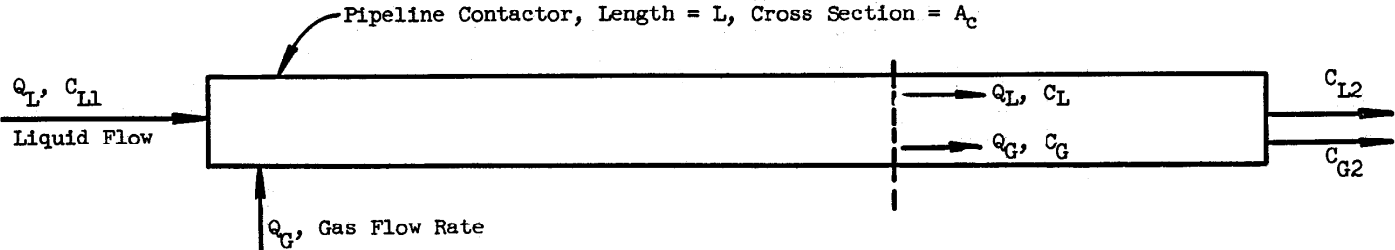
\includegraphics[width=0.77\textwidth]{./images/pipeline_contactor.png}
	\vspace{-2mm}
	\caption{Flow diagram for gas separator (figure reproduced from Peebles 
		\emph{et al.} \cite{peebles_removal_1968}).}
\end{figure}

\end{frame}


\begin{frame}
\frametitle{Fuel processing system overview: TAP concept}
\begin{textblock*}{12.4cm}(0.25cm,1.7cm) % {block width} (coords)
\begin{figure}[htp!] % replace 't' with 'b' to 
	\begin{columns}
		\column{0.65\linewidth}
			\hspace{+3mm}
		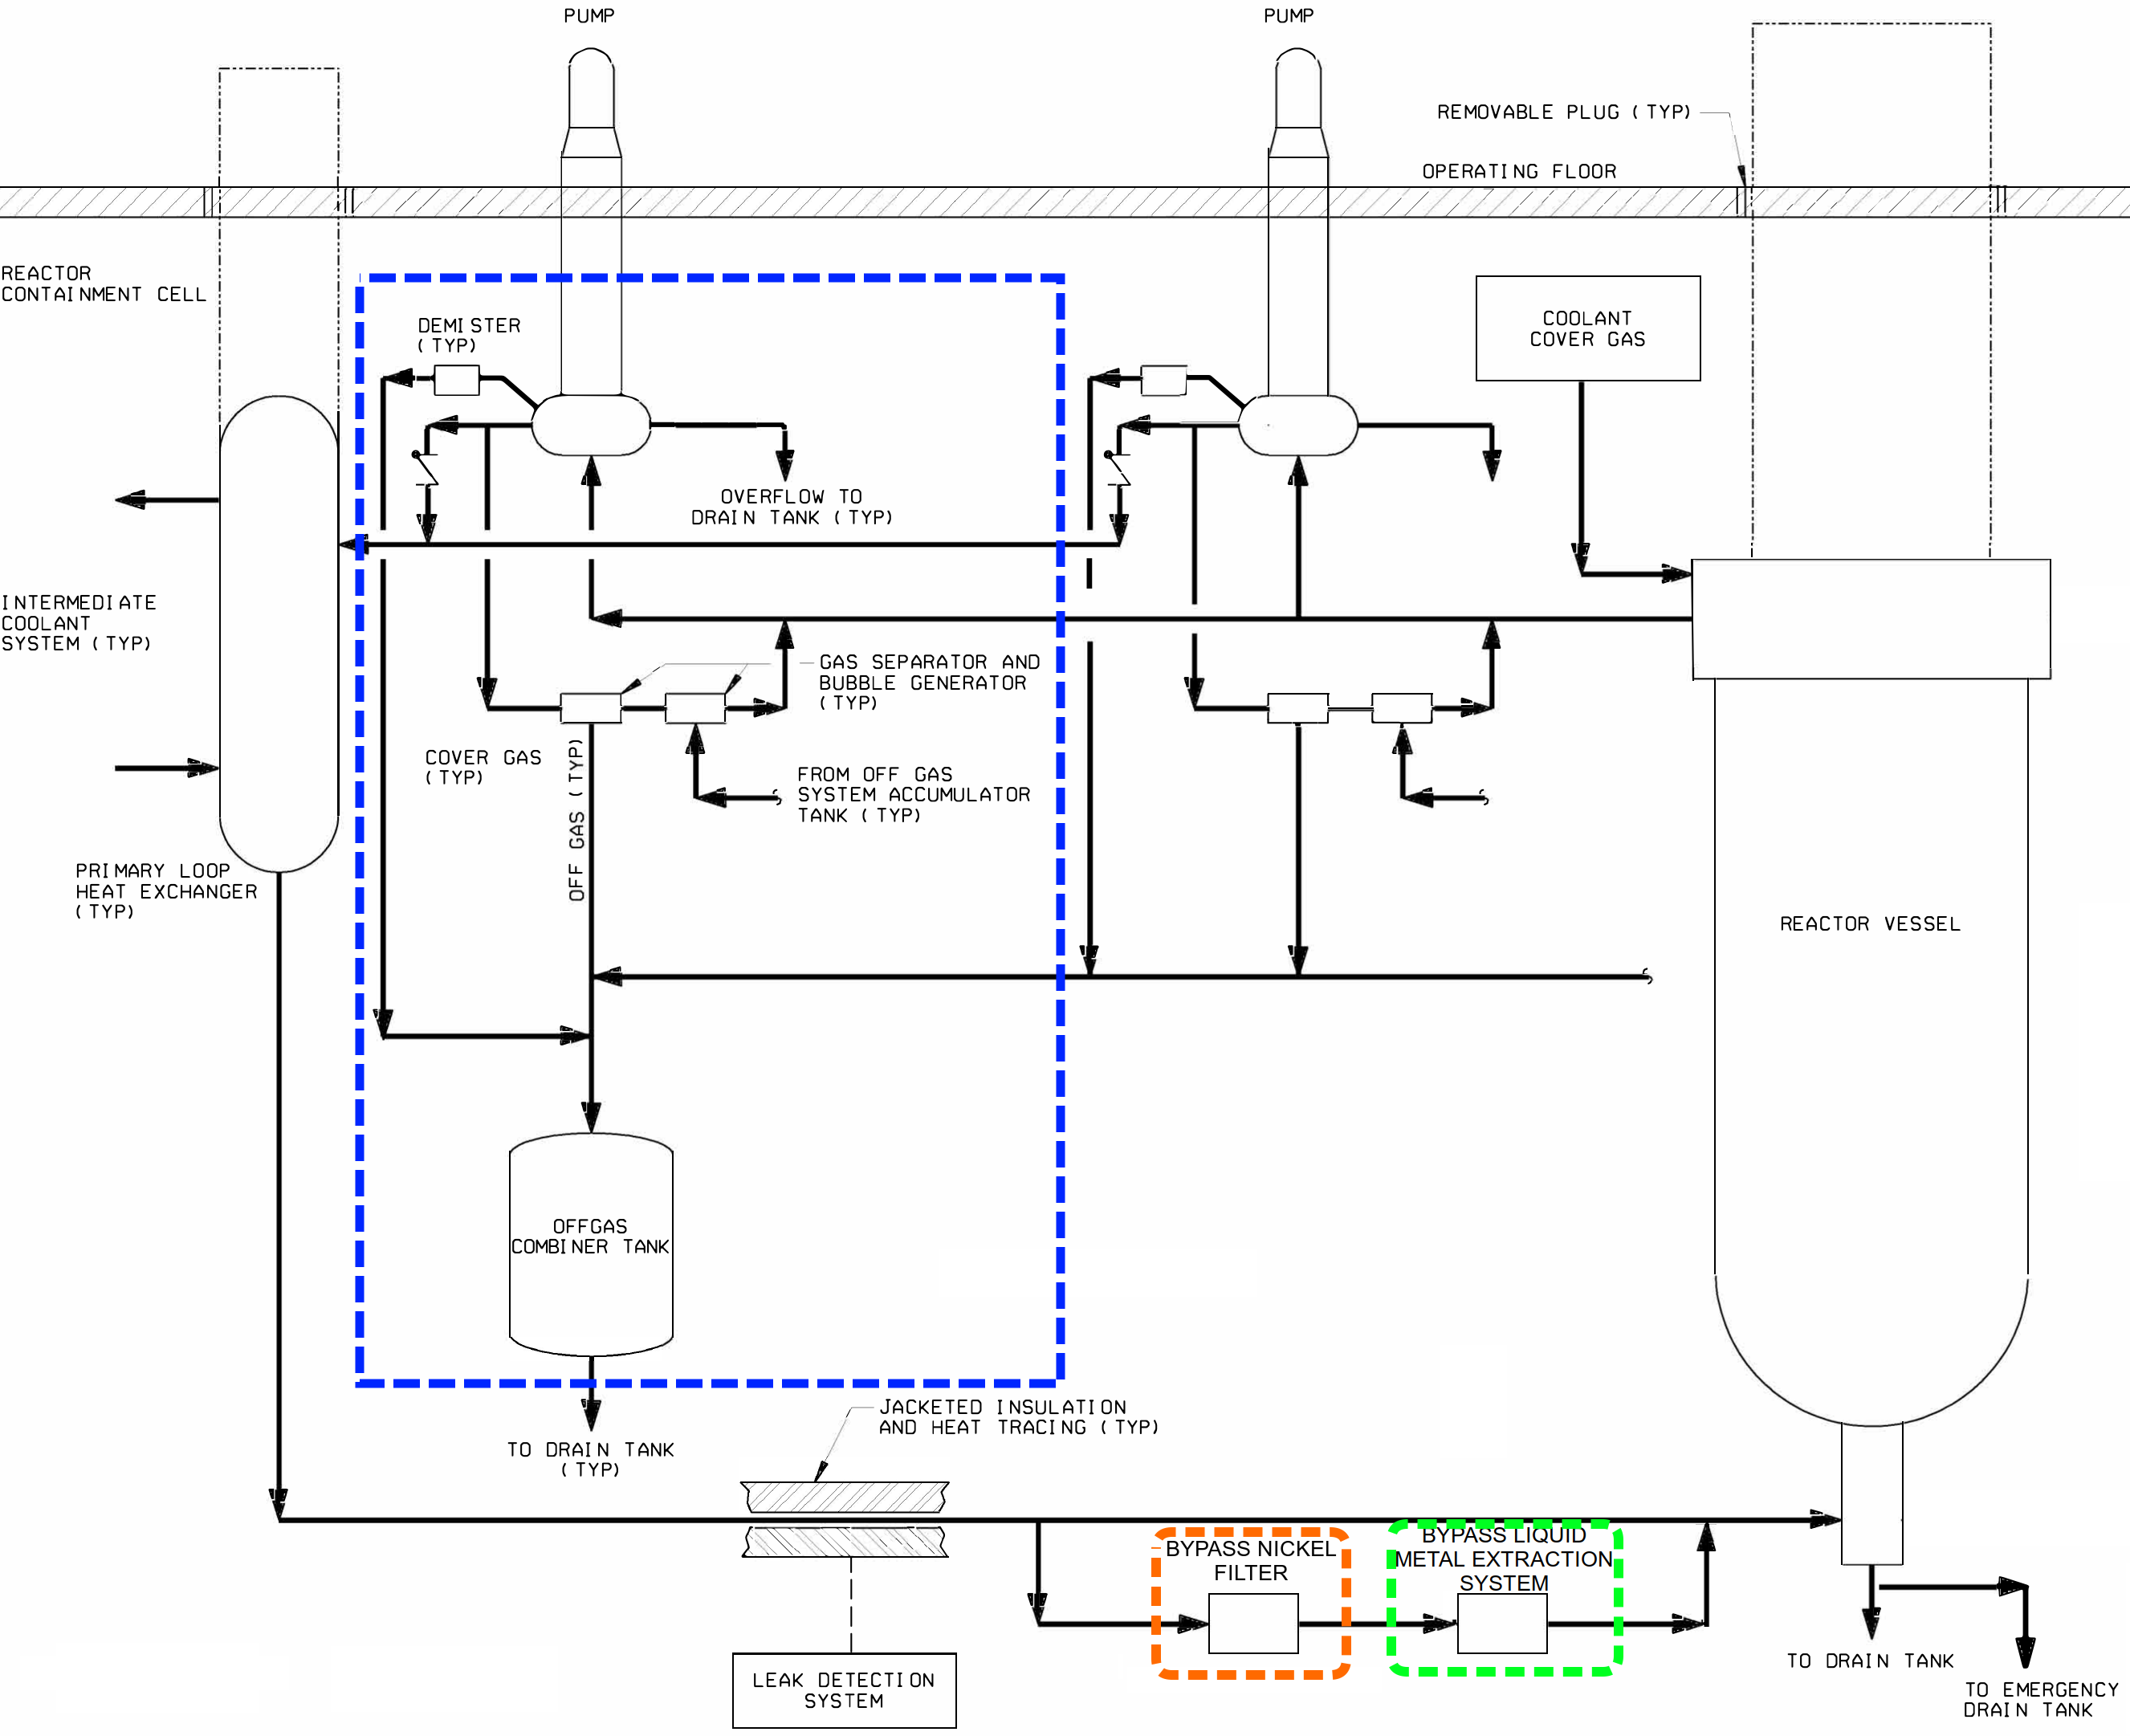
\includegraphics[height=0.88\textheight]{../dissertation/figures/ch4/tap_primary_loop.png}
		
		\column{0.3\linewidth}
		\caption{Simplified \gls{TAP} primary loop design including off-gas 
		system 
		(blue), nickel filter (orange) and liquid metal extraction system 
		(green) \cite{transatomic_power_transatomic_2019}.}
	\end{columns}
\end{figure}
\end{textblock*}
\end{frame}


\subsection{SaltProc tool design}


\begin{frame}
\frametitle{SaltProc class architecture}
	\begin{itemize}
		\item \textit{Simulation} class
			\begin{itemize}
				\item Manages simulation process
				\item Stores data into the HDF5 database
				\item Tracks time, power level
			\end{itemize}
		\item \textit{Depcode} class
			\begin{itemize}
				\item Contains attributes and methods for reading user's input
				\item Creates input files for depletion code
				\item Parses depletion code output 
			\end{itemize}
		\item \textit{Process} class
			\begin{itemize}
				\item Represents fuel processing system component
				\item Contains attributes of the component ($\vec{\epsilon}$, 
				throughput rate)
				\item Tracks waste stream
			\end{itemize}
		\item \textit{MaterialFlow} class
			\begin{itemize}
				\item Instances of that class represents the material flowing between processes
			\end{itemize}
	\end{itemize}
		\vspace{1mm}
	\begin{figure}[ht!] % replace 't' with 'b' to 
		\centering
		\begin{overprint}
		\onslide<1>\centerline{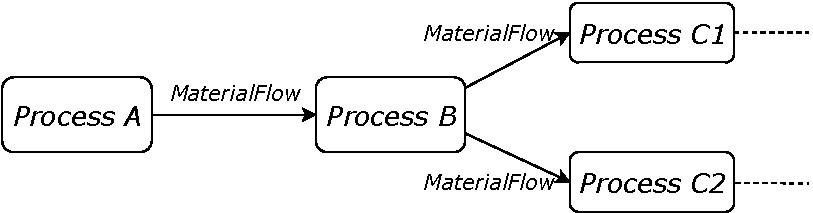
\includegraphics[width=0.6\textwidth]{../dissertation/figures/ch2/materialflow.pdf}}
		\onslide<2>\centerline{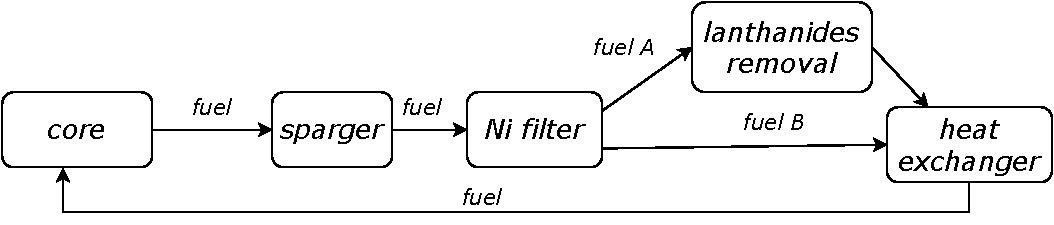
\includegraphics[width=0.6\textwidth]{../dissertation/figures/ch2/tap_materialflow.pdf}}
		\end{overprint}
		\vspace{-2mm}
		\caption{Schematic for passing material data between fuel processing 
		system components.}
	\end{figure}

\end{frame}


\begin{frame}
\frametitle{SaltProc flowchart}
\begin{textblock*}{12.4cm}(0.07cm,1.7cm) % {block width} (coords)
\begin{figure}[ht!] % replace 't' with 'b' to \centering
	\centering
	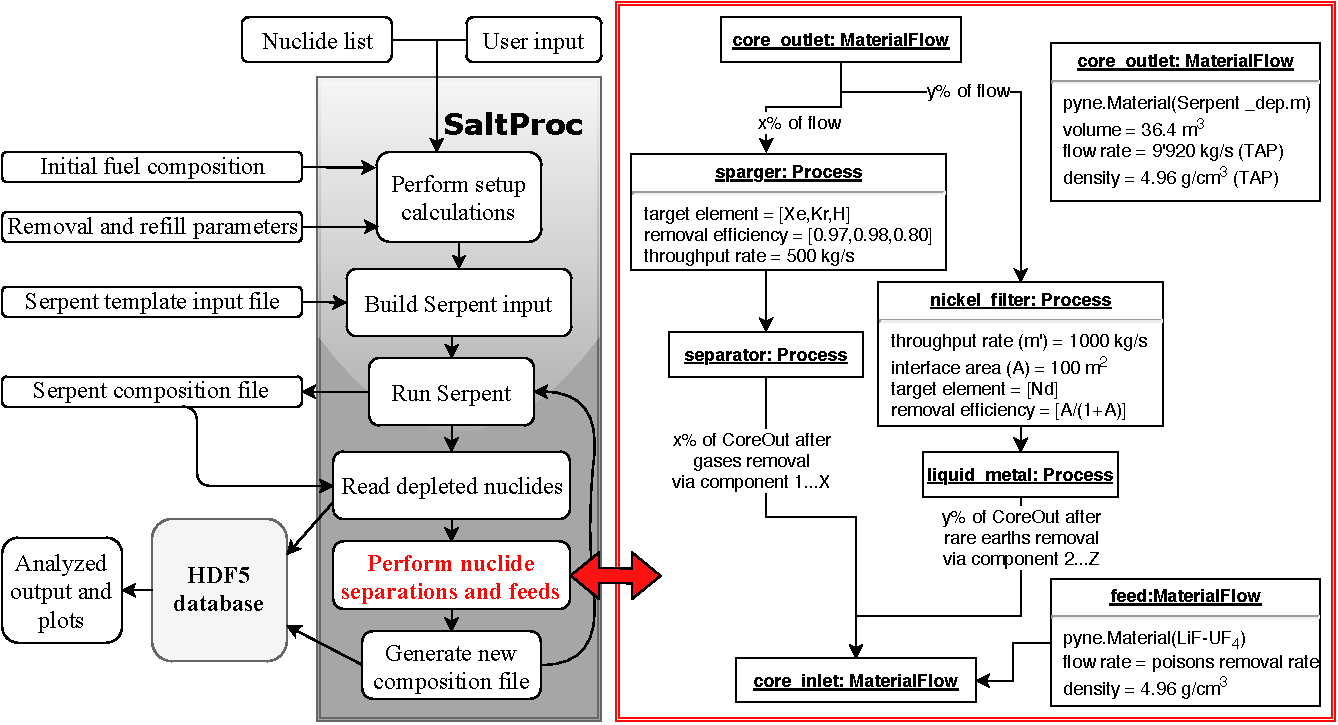
\includegraphics[width=\textwidth]{../dissertation/figures/ch2/saltproc_flowchart.pdf}
		\vspace{-4mm}
	\caption{SaltProc v1.0 Python package flowchart with example of object 
	instances.}
\end{figure}
\end{textblock*}

\end{frame}


\begin{frame}
\frametitle{Multi-component fuel reprocessing system model in SaltProc}       

\begin{figure}[htp!] % replace 't' with 'b' to 
	\centering
	\vspace{-2mm}
	\begin{overprint}
	\onslide<1>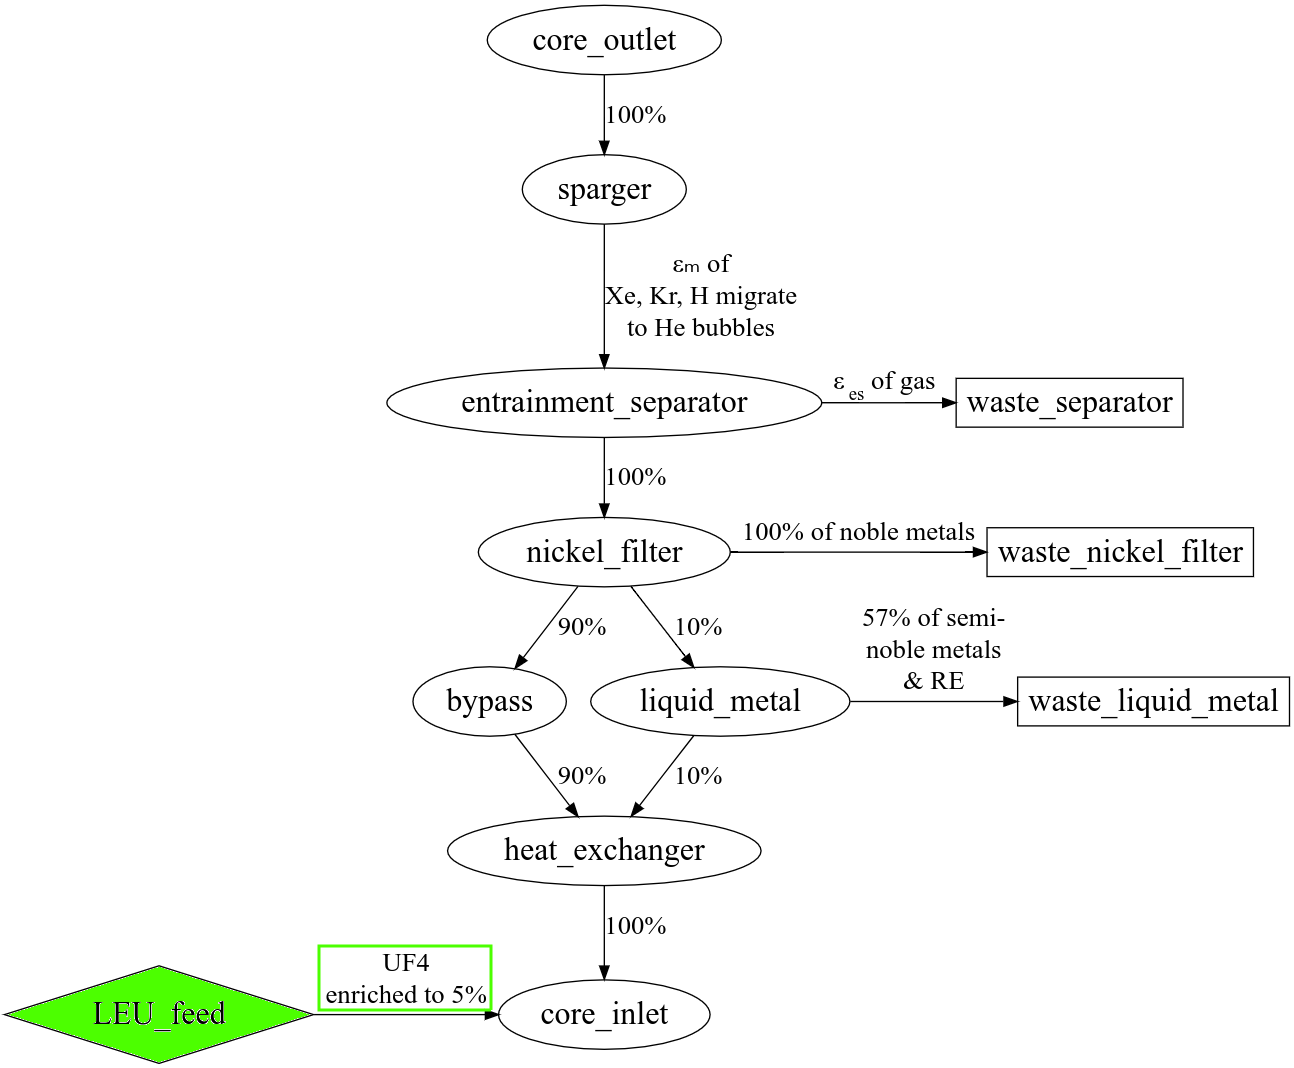
\includegraphics[height=0.85\textheight]{./images/tap_saltproc_var_eps.png}
		\vspace{-2mm}
    \caption{\textcolor{cyan}{\gls{TAP}} reprocessing scheme for 
	SaltProc demonstration.}
	\onslide<2>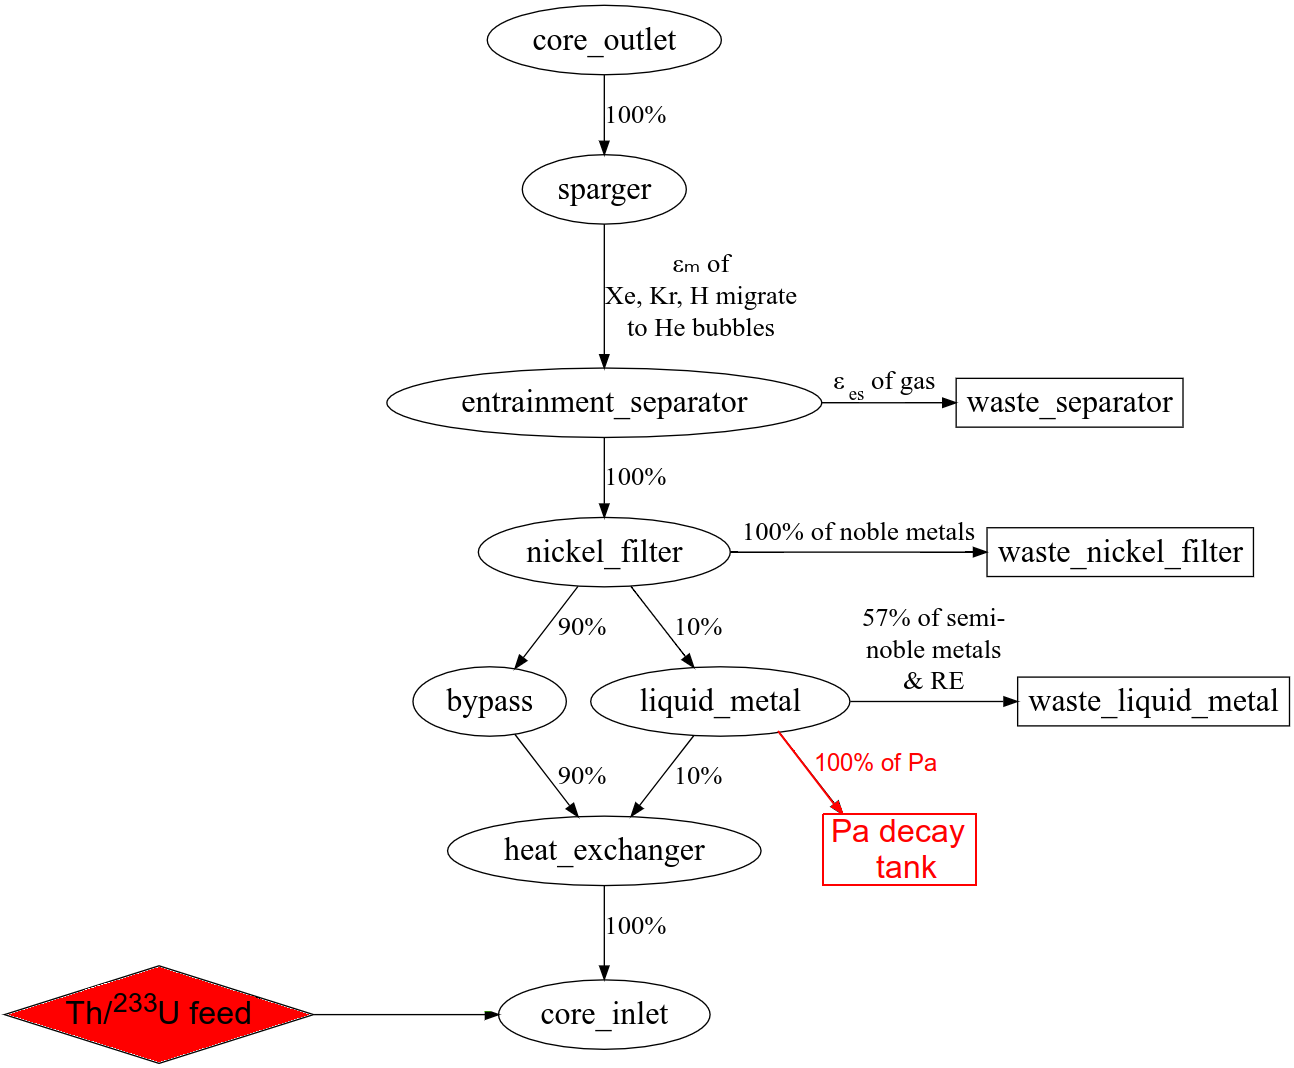
\includegraphics[height=0.85\textheight]{./images/msbr_saltproc_var_eps.png}
		\vspace{-2mm}
	\caption{\textcolor{red}{\gls{MSBR}} reprocessing scheme for 
	SaltProc demonstration.}
	\end{overprint}
\end{figure}

\end{frame}


\begin{frame}[fragile]
\frametitle{DOT-code describing reprocessing system as a directed graph}
\small
\begin{verbatim}
digraph fuel {
==============================================================================
core_outlet -> sparger [label="100%"]
sparger -> waste_sparger [label="60% of Xe, Kr, H"]
sparger -> entrainment_separator [label="100%"]
entrainment_separator -> nickel_filter [label="100%"]
entrainment_separator -> waste_entrainment_separator [label="97% of Xe, Kr, H"]
nickel_filter -> bypass [label="90%"]
bypass -> heat_exchanger [label="90%"]
nickel_filter -> waste_nickel_filter [label="100% of noble metals"]
nickel_filter -> liquid_metal [label="10%"]
liquid_metal -> heat_exchanger [label="10%"]
liquid_metal -> waste_liquid_metal [label="57% of seminoble metals & RE"]
heat_exchanger -> core_inlet [label="100%"]
LEU_feed -> core_inlet
==============================================================================
# Optional parameters to prettify plots
\end{verbatim}
\end{frame}